%% AMS-LaTeX Created with the Wolfram Language : www.wolfram.com

\documentclass{article}
\usepackage{amsmath, amssymb, graphics, setspace}

\newcommand{\mathsym}[1]{{}}
\newcommand{\unicode}[1]{{}}

\begin{document}
\sffamily
\begin{doublespace}
\noindent\(\pmb{A[\text{x$\_$}]\text{:=}\text{Piecewise}[\{\{0.1, 1\leq x<3\}, \{0.5*(x-1),3\leq x\leq 5\}\}];}\\
\pmb{b[\text{x$\_$}]\text{:=}\text{FullSimplify}[\text{Piecewise}[\{\{10, 1\leq x<3\}, \{0,3\leq x\leq 5\}\}] ];}\)
\end{doublespace}

\begin{doublespace}
\noindent\(\pmb{\text{innerIntegral}[\text{r$\_$}]\text{:=} \text{FullSimplify}[\text{Integrate}[b[s],\{s,1,r\},\text{Assumptions}\to 1<r<5]+150*\text{HeavisideTheta}[r-3]];}\)
\end{doublespace}

\begin{doublespace}
\noindent\(\pmb{\text{c1} =\text{FullSimplify}\left[ \frac{\text{NIntegrate}\left[\frac{1}{20*10^6*A[r]}*\text{innerIntegral}[r],\{r,5,1\}\right]}{\text{NIntegrate}\left[\frac{0.1}{A[s]},\{s,5,1\}\right]}\right]}\)
\end{doublespace}

\begin{doublespace}
\noindent\(0.0000377507\)
\end{doublespace}

\begin{doublespace}
\noindent\(\pmb{\text{usol}[\text{x$\_$}]\text{:=}\text{FullSimplify}\left[-\text{Integrate}\left[\frac{1}{20*10^6*A[r]}*\text{innerIntegral}[r],\{r,5,x\},\text{Assumptions}\to
1\leq x\leq 5\right]+\right.}\\
\pmb{\left.\text{c1}*\text{Integrate}\left[\frac{1}{A[s]},\{s,5,x\},\text{Assumptions}\to 1\leq x\leq 5\right]\right];}\)
\end{doublespace}

\begin{doublespace}
\noindent\(\pmb{\text{ue} = \text{FullSimplify}[\text{usol}[x]];}\)
\end{doublespace}

\begin{doublespace}
\noindent\(\pmb{\text{Plot}[\text{ue},\{x,1,5\}]}\)
\end{doublespace}

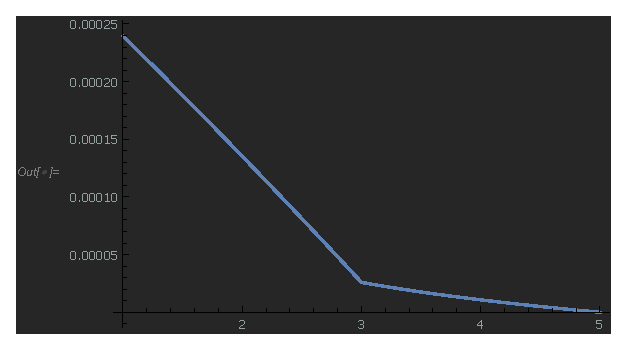
\includegraphics{AnalyticalHW4_gr1.eps}

\begin{doublespace}
\noindent\(\pmb{\text{inn} = \text{innerIntegral}[x];}\)
\end{doublespace}

\begin{doublespace}
\noindent\(\pmb{\text{Plot}[\text{inn},\{x,1,5\}]}\)
\end{doublespace}

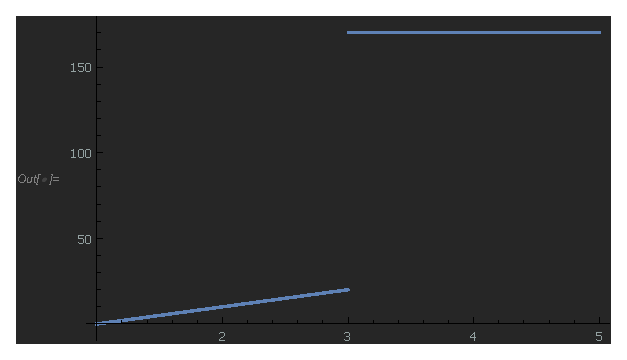
\includegraphics{AnalyticalHW4_gr2.eps}

\end{document}
